\chapter{Grundlagen}\label{chp:Grundlageb}
In diesem Kapitel werden die Grundlagen beschrieben

%%%%%%%%%%%%%%%%%%%%%%%%%%%%%%%%%%%%%%%%%%%%%%%%%%%%%%%%%%%%%%%%%%%%%%%%%%%%%%%%%%%%%%%%%%%%%%%
\section{Grundlage 1}\label{sec:Grundlage1}
\subsection{subsection}
text

\section{CPACS}

\section{Airfoils}
Wie schon in Kapitel~\ref{sec:Grundlage1} beschrieben ...

\begin{figure}[htpb]
	\centering
		\begin{figure}[htpb]
	\centering
\beginpgfgraphicnamed{profile-f1}
\footnotesize
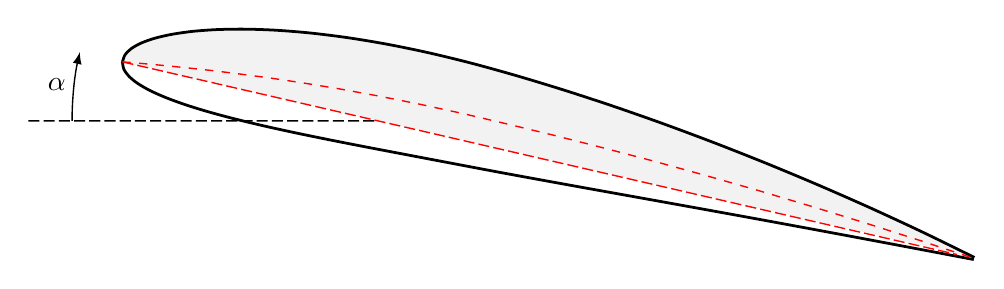
\begin{tikzpicture}[>=latex,scale=1.11]
\tikzstyle{spring}=[snake=zigzag,thick,line before snake=0.3cm,line after  snake=0.3cm,segment length=6,segment amplitude=5,join=round]%
\begin{scope}[rotate around={-13:(10,0)}]
% bottom_second
\draw[smooth,line width=1pt] plot coordinates {(0,0)(0.0334,-0.0767)(0.1087,-0.1437)(0.2253,-0.2011)(0.3824,-0.2489)(0.5790,-0.2870)(0.8139,-0.3158)(1.0860,-0.3355)(1.3940,-0.3466)(1.7365,-0.3497)(2.1123,-0.3457)(2.5199,-0.3356) (2.9580,-0.3209)(3.4252,-0.3029)(3.9198,-0.2835)(4.4427,-0.2625)(4.9936,-0.2377)(5.5666,-0.2102)(6.1594,-0.1810)(6.7696,-0.1513)(7.3950,-0.1217)(8.0332,-0.0930)(8.6815,-0.0653)(9.3376,-0.0386)(9.9988,-0.0125)};
% top_first
\draw[smooth,line width=1pt,fill=black!5] plot coordinates {(0,0)(0.0095,0.0831)(0.0624,0.1691)(0.1590,0.2574)(0.2990,0.3467)(0.4824,0.4357)(0.7085,0.5225)(0.9765,0.6050)(1.2855,0.6812)(1.6341,0.7488)(2.0206,0.8055)(2.4433,0.8492)(2.8998,0.8778)(3.3879,0.8897)(3.9049,0.8833)(4.4459,0.8592)(5.0064,0.8210)(5.5876,0.7687)(6.1870,0.7023)(6.8016,0.6219)(7.4286,0.5277)(8.0650,0.4197)(8.7080,0.2980)(9.3544,0.1623)(10.0012,0.0125)};
% sekelett
\draw[dashed, color=red, line width=0.5pt] plot coordinates { (0.0, 0.0)(0.021, 0.003)(0.086, 0.013)(0.192, 0.028)(0.341, 0.049)(0.531, 0.074)(0.761, 0.103)(1.031, 0.135)(1.34, 0.167)(1.685, 0.2)(2.066, 0.23)(2.482, 0.257)(2.929, 0.278)(3.407, 0.293)(3.912, 0.3)(4.444, 0.298)(5.0, 0.292)(5.577, 0.279)(6.173, 0.261)(6.786, 0.235)(7.412, 0.203)(8.049, 0.163)(8.695, 0.116)(9.346, 0.062)(10.0, 0.0) };
\draw[line width=0.5pt,dashed,dash pattern=on 4pt off 1.5pt,rotate around={13:(3,0)}](-1,0)--(3,0);
% arrows
\draw[line width=0.5pt,<-](3,0) +(180:3.5cm) arc (180:193:3.5cm);
\draw(3,0) +(186.5:3.7cm) node{$\alpha$};
% sehne
\draw[line width=0.5pt,color=red, dashed,dash pattern=on 4pt off 1.5pt](0,0)--(9.8,0);
\end{scope}%
\end{tikzpicture}
\endpgfgraphicnamed%



\begin{tikzpicture}
% profile with data file
%\newcounter{y}
\setcounter{y}{0}
\foreach \x in {1.00}
    \draw (11 cm,1pt) -- (11 cm,-1pt) node[anchor=north] {$\x$};
    \draw (1pt,0 cm) -- (-1pt,0 cm) node[anchor=east] {$0$};
	\draw (1pt,1.25 cm) -- (-1pt,1.25 cm) node[anchor=east] {$0.10$};
	\draw (1pt,-1.25 cm) -- (-1pt,-1.25 cm) node[anchor=east] {$-0.10$};
    \foreach \lbl / \fn in {naca4815.dat}{
        % Some profiles look better when using plot[smooth]
        \draw[yshift=-\arabic{y}cm,scale=11, fill=black!5]% node[left=0.5cm] {\lbl}
            plot file{tikz/data/\fn} -- cycle;
        \stepcounter{y}
    }
% axis
\draw[thick,-] (0,0)  -- (12,0) node[anchor=west] {x};
\draw[thick,-] (0,-2) -- (0,2) node[anchor=south] {y};    
% camber line    
\draw[smooth, dashed, scale=11] plot coordinates {(1.0,0.0)(0.998459,0.000614)(0.993844,0.0024245)(0.986185,0.0053355)(0.975528,0.00919)(0.96194,0.0137755)(0.945503,0.018829)(0.92632,0.0240435)(0.904508,0.029078)(0.880203,0.0335675)(0.853553,0.037132)(0.824724,0.039389)(0.793893,0.0399975)(0.761249,0.0399065)(0.726995,0.039667)(0.691342,0.039262)(0.654508,0.038677)(0.616723,0.037901)(0.578217,0.036926)(0.53923,0.03575)(0.5,0.034375)(0.46077,0.0328075)(0.421783,0.0310595)(0.383277,0.0291465)(0.345492,0.0270885)(0.308658,0.0249115)(0.273005,0.022642)(0.238751,0.0203125)(0.206107,0.0179555)(0.175276,0.0156075)(0.146447,0.013304)(0.119797,0.0110825)(0.095492,0.008979)(0.07368,0.0070285)(0.054497,0.005264)(0.03806,0.0037155)(0.024472,0.0024095)(0.013815,0.0013695)(0.006156,0.000613)(0.001541,0.000154)(0.0,0.0)};    	
\end{tikzpicture}    


\begin{tikzpicture}
% axis
\draw[thick,-] (11,0)  -- (12,0) node[anchor=west] {x};
\draw[thick,-] (0,-2) -- (0,2) node[anchor=south] {y};
% profile with data file
%\newcounter{y}
\setcounter{y}{0}
\foreach \x in {1.00}
    \draw (11 cm,1pt) -- (11 cm,-1pt) node[anchor=north] {$\x$};
    \draw (1pt,0 cm) -- (-1pt,0 cm) node[anchor=east] {$0$};
	\draw (1pt,1.25 cm) -- (-1pt,1.25 cm) node[anchor=east] {$0.10$};
	\draw (1pt,-1.25 cm) -- (-1pt,-1.25 cm) node[anchor=east] {$-0.10$};
    \foreach \lbl / \fn in {naca4815.dat}{
        % Some profiles look better when using plot[smooth]
        \draw[yshift=-\arabic{y}cm,scale=11]% node[left=0.5cm] {\lbl}
            plot file{tikz/data/\fn} -- cycle;
        \stepcounter{y}
    }
% camber line    
\draw[smooth, dashed, color=red, scale=11] plot coordinates {(1.0,0.0)(0.998459,0.000614)(0.993844,0.0024245)(0.986185,0.0053355)(0.975528,0.00919)(0.96194,0.0137755)(0.945503,0.018829)(0.92632,0.0240435)(0.904508,0.029078)(0.880203,0.0335675)(0.853553,0.037132)(0.824724,0.039389)(0.793893,0.0399975)(0.761249,0.0399065)(0.726995,0.039667)(0.691342,0.039262)(0.654508,0.038677)(0.616723,0.037901)(0.578217,0.036926)(0.53923,0.03575)(0.5,0.034375)(0.46077,0.0328075)(0.421783,0.0310595)(0.383277,0.0291465)(0.345492,0.0270885)(0.308658,0.0249115)(0.273005,0.022642)(0.238751,0.0203125)(0.206107,0.0179555)(0.175276,0.0156075)(0.146447,0.013304)(0.119797,0.0110825)(0.095492,0.008979)(0.07368,0.0070285)(0.054497,0.005264)(0.03806,0.0037155)(0.024472,0.0024095)(0.013815,0.0013695)(0.006156,0.000613)(0.001541,0.000154)(0.0,0.0)};  
% sehne
\draw[line width=0.5pt,color=red](0,0)--(11,0);    	
\end{tikzpicture} 
	\caption{Eine Vektorgrafik}
	\label{fig:vectorExample}
\end{figure}









	\caption{Eine Vektorgrafik}
	\label{fig:vectorExample}
\end{figure}


\section{Flugzeug}
text